%% ================================================================
%% Artículo del proyecto de grado - Maestría en Inteligencia Artificial
%% Universidad de los Andes - Curso Proyecto: despliegue de soluciones
%% Plantilla: IEEEtran.cls v1.7a (modo conference)
%% ================================================================

\documentclass[conference,letterpaper]{IEEEtran}

\usepackage[T1]{fontenc}
\usepackage[utf8]{inputenc}
\usepackage{mathptmx}
\usepackage[spanish,es-tabla,es-nodecimaldot,es-noshorthands]{babel}
\usepackage{icomma}
\usepackage{microtype}
\usepackage{amsmath,amssymb}
\usepackage{graphicx}
\usepackage{booktabs}
\usepackage{array}
\usepackage{multirow}
\usepackage{url}
\usepackage[hidelinks]{hyperref}

\renewcommand{\figurename}{Figura}
\renewcommand{\tablename}{Tabla}
\renewcommand{\refname}{Referencias}
\renewcommand{\abstractname}{Resumen}

\title{Sistema de Alertas Clínicas Tempranas con IA Interpretable para la Predicción de Riesgos en Niños Prematuros y de Bajo Peso del Programa Madre Canguro}

\author{
\IEEEauthorblockN{Alex Paul Chirino Caicedo, Breitner Enrique González, Santiago José Ramos Echeverry, Wilfrido Alberto Gómez Pérez}
\IEEEauthorblockA{Universidad de los Andes -- Fundación Canguro\\
Maestría en Inteligencia Artificial\\
Octubre de 2026}
}

\begin{document}
\maketitle

\begin{abstract}
Se presenta una solución de inteligencia artificial interpretable para apoyar la revisión de registros longitudinales y la estimación de riesgos en niños prematuros o de bajo peso vinculados al Programa Madre Canguro. La propuesta integra un componente de control de calidad y detección de anomalías con modelos de riesgo clínico calibrados y explicables. El sistema no sustituye la valoración médica: organiza datos, prioriza registros para revisión y produce estimaciones probabilísticas acompañadas de explicaciones. La arquitectura contempla procesamiento interno de datos reales y una demostración pública con datos simulados, manteniendo separación entre ambientes y trazabilidad de los experimentos.
\end{abstract}

\section{Descripción breve de la propuesta de solución}
La solución responde a dos dificultades complementarias: la calidad variable de los registros clínicos y la necesidad de anticipar desenlaces antes de la siguiente visita. Se implementan dos modelos encadenados. El primero evalúa conformidad y plausibilidad de los datos mediante reglas, modelos contextuales y comparaciones longitudinales. El segundo utiliza la información disponible hasta un corte de seguimiento para estimar riesgos clínicos por desenlace.

El umbral que transforma una probabilidad en una alerta pertenece a la aplicación y a la gobernanza clínica, no al entrenamiento del clasificador. Esta separación permite distinguir errores de captura de señales potencialmente clínicas y conservar trazabilidad sobre las decisiones.

El alcance operativo se ajustó a una ejecución alineada con la carga semestral de la fuente institucional, manteniendo inferencia a demanda y separación entre datos reales y simulados. El despliegue contempla registro de modelos, API de inferencia y tablero web.

\begin{figure}[!t]
    \centering
    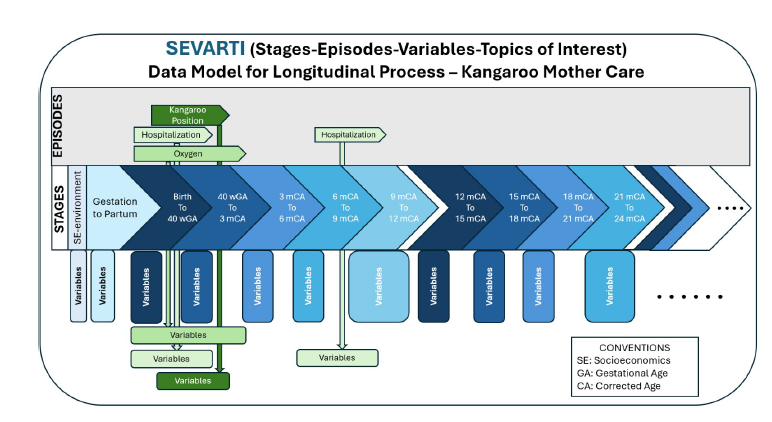
\includegraphics[width=\columnwidth]{figuras/figura1_sevarti.png}
    \caption{Modelo conceptual SEVARTI: etapas, episodios y variables.}
    \label{fig:sevarti}
\end{figure}

\section{Recolección y preparación de los datos}
\subsection{Fuente, extracción y contrato de datos}
SEVARTI (\textit{Stages--Episodes--Variables--Topics of Interest}) organiza procesos longitudinales mediante etapas de desarrollo, episodios de atención y variables asociadas a cada momento. En el Programa Madre Canguro permite ubicar controles y antecedentes sobre un eje de edad gestacional o corregida, diferenciando visitas programadas de episodios con duración propia.

Los registros provienen de una capa de consumo PostgreSQL institucional consultada con permisos de solo lectura. El corte documentado corresponde al 24 de julio de 2026. El universo reportado contiene 62\,043 pacientes y aproximadamente 13,9 millones de mediciones. El adaptador representa la información mediante seis entidades: esquema, etapas, sujetos, mediciones, episodios y quiebres históricos.

El corte principal documenta 339 variables catalogadas, 318 de ellas en uso. Dado que versiones previas del diccionario difieren en el número total de variables, cada experimento debe conservar el identificador de la versión utilizada.

La partición experimental se realizó por niño y año de nacimiento, separando los regímenes anteriores y posteriores al cambio de registro de 2022. Para anomalías se reportaron 40\,711 niños en entrenamiento, 7\,330 en calibración y 8\,955 en prueba. Para clasificación clínica se reportaron 48\,041 en entrenamiento y 8\,955 en prueba.

\subsection{Edad corregida, consistencia y faltantes}
La edad corregida en días se calculó mediante
\begin{equation}
EC = \text{edad posnatal (días)} - 7(40-\text{EG}),
\end{equation}
donde EG es la edad gestacional en semanas.

Se verificaron fechas de nacimiento y visita, edades consignadas, orden temporal, unidades y ventanas de seguimiento. Los valores dudosos se marcan para revisión y, según el protocolo, se excluyen como objetivos válidos o se representan como faltantes; no se sustituyen automáticamente por estimaciones.

La auditoría identificó códigos de relleno no documentados, unidades inconsistentes, fechas imposibles y cambios de codificación alrededor de 2022. También se observó pérdida de seguimiento: la cobertura de peso se aproxima al 78\,\% en 40 semanas y al 49\,\% a los 12 meses de edad corregida.

\begin{figure}[!t]
    \centering
    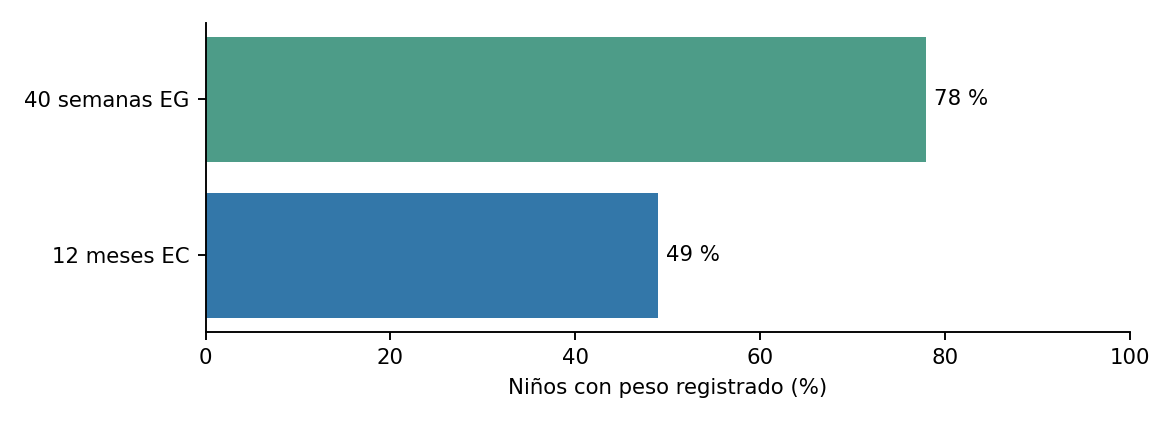
\includegraphics[width=\columnwidth]{figuras/figura2_cobertura_peso.png}
    \caption{Cobertura de peso en dos controles para el corte analizado.}
    \label{fig:cobertura}
\end{figure}

\section{Construcción de los modelos y solución}
\subsection{Flujo reproducible y control de versiones}
El pipeline integra preparación SEVARTI, validación del diccionario, detección de anomalías, construcción de variables clínicas, entrenamiento por desenlace, evaluación y cálculo de riesgos. Los resultados, modelos y artefactos se versionan para conservar reproducibilidad y permitir comparación entre cortes.

\subsection{Modelo de anomalías}
La detección se organiza en cinco niveles: contrato, valor, contexto, trayectoria y grupo-tiempo. La revisión robusta utiliza
\begin{equation}
z_r = \frac{x-\mathrm{mediana}}{1.4826\,\mathrm{MAD}},
\end{equation}
y marca candidatos cuando $|z_r|>3.5$.

En la capa contextual se ajustan modelos LightGBM cuantílicos para $Q_{0.25}$, $Q_{0.50}$ y $Q_{0.75}$. El residuo estandarizado se contrasta con un umbral conformal obtenido en calibración con $\alpha=0.005$. La capa temporal agrega indicadores trimestrales y CUSUM para vigilar cambios sistemáticos.

\begin{table}[!t]
\caption{Niveles de revisión de anomalías}
\label{tab:anomalias}
\centering
\footnotesize
\begin{tabular}{p{0.14\columnwidth} p{0.35\columnwidth} p{0.38\columnwidth}}
\toprule
Nivel & Procedimiento & Propósito \\
\midrule
0 & Tipo, unidad y tiempo & Validar contrato \\
1 & Estadísticos robustos & Detectar extremos \\
2 & LightGBM cuantílico & Revisar contexto \\
3 & Cambios entre visitas & Detectar saltos \\
4 & Indicadores temporales & Detectar deriva \\
\bottomrule
\end{tabular}
\end{table}

\subsection{Clasificación de riesgos y explicabilidad}
Para cada desenlace y corte se construyen firmas con antecedentes basales, historia de visitas, episodios y mediciones conocidas hasta ese instante. Los clasificadores LightGBM producen probabilidades que se calibran mediante regresión isotónica y se comparan con reglas simples.

Las explicaciones locales se obtienen con TreeSHAP para identificar contribuciones de variables sin atribuir causalidad. La partición por paciente y la separación cronológica son indispensables para evitar fuga de información.

Se documentaron 14 desenlaces modelados: cinco ventanas de readmisión, cinco de inasistencia a la siguiente visita, dos de oxigenodependencia y dos de desarrollo psicomotor bajo. Los desenlaces antropométricos a 12 meses se consideran una extensión diferenciada.

\subsection{Trayectorias antropométricas}
La trayectoria antropométrica se define como la sucesión ordenada de peso, talla y perímetro cefálico con edades reales y eventos asociados. Se consideran nivel, dirección, velocidad y cambios de pendiente, preferiblemente mediante puntajes $z$ apropiados para sexo y edad corregida.

Se definieron hitos de nacimiento, inicio y salida de posición canguro, 40 semanas y controles de 3, 6, 9 y 12 meses de edad corregida. Para predicción a 12 meses se compararán firmas en 40 semanas, 3, 6 y 9 meses.

\subsection{Arquitectura técnica y protección de datos}
El procesamiento de datos reales se mantiene en un equipo local con GPU y acceso de solo lectura a PostgreSQL institucional. El entorno incorpora CLI de entrenamiento, MLflow para seguimiento experimental, MinIO para artefactos, PostgreSQL local, FastAPI para inferencia y React/nginx para visualización.

La demostración pública desplegada en Railway utiliza únicamente datos simulados y un paquete de modelo destinado a ese propósito. Los datos e inferencias individuales reales permanecen en el entorno autorizado.

\begin{figure}[!t]
    \centering
    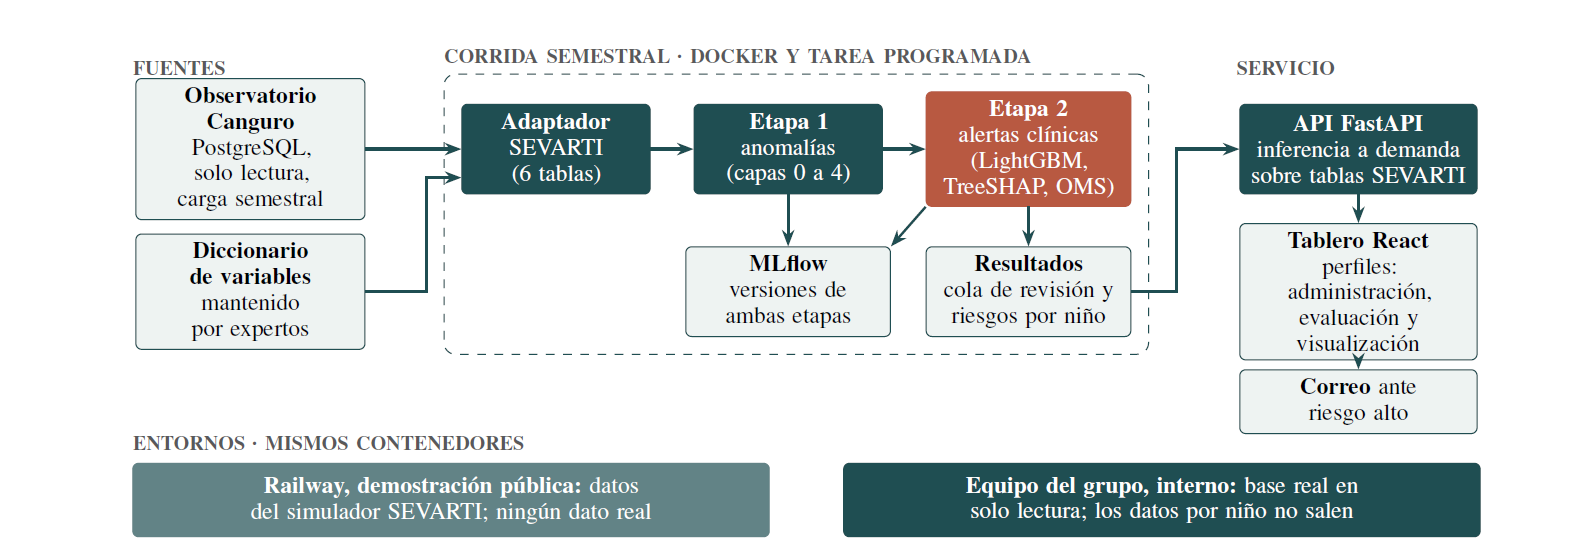
\includegraphics[width=\columnwidth]{figuras/figura3_arquitectura.png}
    \caption{Arquitectura lógica del sistema: SEVARTI, anomalías, riesgos y servicio.}
    \label{fig:arquitectura}
\end{figure}

\section{Resultados obtenidos}
La validación interna de los 14 desenlaces mostró que 13 comparaciones de AUROC favorecen al modelo frente a la regla simple. Para oxigenodependencia a tres meses se obtuvo AUROC de 0.91 frente a 0.80 de la regla. El 67.7\,\% de los casos se concentró en el decil de mayor riesgo, frente a 49.3\,\% para la referencia simple.

El detector de anomalías alcanzó una detección global documentada del 75.3\,\% sobre seis clases de perturbaciones sintéticas, con 18.8 alertas por cada 1\,000 registros sin perturbación. En desviaciones de tres desviaciones estándar la detección fue de 78\,\% frente a 27\,\% con la regla simple; en alteraciones de etapa fue de 68\,\% frente a 5\,\%.

Estos resultados corresponden a experimentos retrospectivos internos. No constituyen validación prospectiva definitiva, validación externa ni aprobación clínica del sistema.

\section{Análisis, retos y próximos pasos}
La lectura conjunta de discriminación y calibración es esencial: un clasificador puede ordenar correctamente el riesgo y, al mismo tiempo, sobreestimar probabilidades. Los desenlaces de inasistencia presentan discriminación moderada y requieren evaluación por desenlace con intervalos de confianza, precisión--recall y utilidad operativa.

La pérdida de seguimiento es un riesgo metodológico central. Por ello, las firmas incrementales deben utilizar la información disponible hasta cada corte y documentar patrones de ausencia. También se requiere controlar los cambios de captura alrededor de 2022 para evitar confundir deriva de registro con cambios clínicos.

Como siguientes acciones se propone: congelar la versión del corte y del diccionario; completar auditorías por desenlace y subgrupo; generar curvas de calibración e intervalos de confianza; implementar firmas incrementales en 40 semanas, 3, 6 y 9 meses; revisar muestras ciegas con expertos clínicos; y contrastar predicciones guardadas contra un corte posterior cuando esté disponible.

\section{Conclusiones}
La propuesta integra control de calidad, detección de anomalías, predicción clínica interpretable y despliegue reproducible. Los resultados retrospectivos sugieren que el contexto longitudinal aporta información adicional frente a reglas simples, pero la utilidad clínica requiere validación temporal y revisión experta. La separación entre datos reales y simulados, el acceso de solo lectura y el versionamiento de modelos y artefactos constituyen elementos centrales de la arquitectura.

\begin{thebibliography}{00}
\bibitem{villar2015} J. Villar et al., ``Postnatal growth standards for preterm infants,'' \textit{The Lancet Global Health}, vol. 3, no. 11, pp. e681--e691, 2015, doi: 10.1016/S2214-109X(15)00163-1.
\bibitem{fenton2013} T. R. Fenton and J. H. Kim, ``A systematic review and meta-analysis to revise the Fenton growth chart for preterm infants,'' \textit{BMC Pediatrics}, vol. 13, art. 59, 2013, doi: 10.1186/1471-2431-13-59.
\bibitem{tripod2024} G. S. Collins et al., ``TRIPOD+AI statement: updated guidance for reporting clinical prediction models that use regression or machine learning methods,'' \textit{BMJ}, vol. 385, e078378, 2024, doi: 10.1136/bmj-2023-078378.
\bibitem{lightgbm2017} G. Ke et al., ``LightGBM: A highly efficient gradient boosting decision tree,'' in \textit{Advances in Neural Information Processing Systems}, vol. 30, 2017.
\bibitem{shap2017} S. M. Lundberg and S.-I. Lee, ``A unified approach to interpreting model predictions,'' in \textit{Advances in Neural Information Processing Systems}, vol. 30, 2017.
\bibitem{who2022} World Health Organization, \textit{WHO Recommendations for Care of the Preterm or Low-Birth-Weight Infant}. Geneva, Switzerland: WHO, 2022.
\end{thebibliography}

\end{document}
